% for sharelatex https://www.sharelatex.com/github/
% !TEX program = pdflatex

\documentclass[hyper]{tufte-handout}
\usepackage{morefloats}

% \providecommand{\url}[1]{\texttt{#1}}
% \providecommand{\urlprefix}{URL }
% \expandafter\ifx\csname urlstyle\endcsname\relax
%   \providecommand{\doi}[1]{doi:\discretionary{}{}{}#1}\else
%   \providecommand{\doi}{doi:\discretionary{}{}{}\begingroup
%   \urlstyle{rm}\Url}\fi
% \providecommand{\bibAnnoteFile}[1]{%
%   \IfFileExists{#1}{\begin{quotation}\noindent\textsc{Key:} #1\\
%   \textsc{Annotation:}\ \input{#1}\end{quotation}}{}}
% \providecommand{\bibAnnote}[2]{%
%   \begin{quotation}\noindent\textsc{Key:} #1\\
%   \textsc{Annotation:}\ #2\end{quotation}}
% \providecommand{\eprint}[2][]{\url{#2}}


% Set up the images/graphics package
\usepackage{graphicx}
\setkeys{Gin}{width=\linewidth,totalheight=\textheight,keepaspectratio}
\graphicspath{{figures/}}

% The following package makes prettier tables.  We're all about the bling!
%\usepackage{booktabs}

% The units package provides nice, non-stacked fractions and better spacing
% for units.
% \usepackage{units}

% The fancyvrb package lets us customize the formatting of verbatim
% environments.  We use a slightly smaller font.
% \usepackage{fancyvrb}
% \fvset{fontsize=\normalsize}

% Small sections of multiple columns
% \usepackage{multicol}


\hypersetup{colorlinks}

% https://en.wikibooks.org/wiki/LaTeX/Hyperlinks#.5Chyperref
% http://www.tug.org/applications/hyperref/manual.html#x1-120003.8
% \hypersetup{
%     pdfauthor={},
%     pdftitle={Tufte-LaTeX document},
%     pdfsubject={subject},
%     pdfkeywords={}
% }
% \href{http://example.com}{test}
% \href{http://www.wikibooks.org}{Wikibooks home}
% http://tex.stackexchange.com/questions/66526/what-is-the-right-way-to-use-hyperref-options-with-tufte-handout-class

\newcommand{\etal}{\textit{et. al.}}
%\newcommand{\scite}[3]{\sidenote{#1 \etal\ #2, \url{#3}}}
%\newcommand{\scite}[3]{(#1 \etal\ #2)\sidenote{\url{#3}}}
\newcommand{\scite}[3]{\sidenote{\href{#3}{#1 \etal\ #2.}}}

\title{Research Statement}
\author{Frederick Matsen, Fred Hutchinson Cancer Research Center} % \thanks{\url{http://matsen.fhcrc.org/}}}


\begin{document}

\maketitle

\begin{abstract}
\noindent
The research questions I enjoy most mix mathematical, statistical, and computational thinking to answer a question that either brings new insight to a biological problem, or provides novel methodology that is needed for a class of biological problems.
Specifically, while at the Center my work has been in the intersection of evolutionary molecular sequence analysis and biomedicine.
I have especially focused on methods that that integrate out uncertainty using a likelihood-based framework, or leverage hidden structure to the data.
\end{abstract}





% I will begin by introducing a few of the concepts that are necessary to frame the work.
\newthought{Model-based statistical inference provides a unified framework} to learn from plentiful, indirect, and often noisy biological data.\sidenote{%
Here \textit{model-based} means that our ideas about how the system works are formalized into a probabilistic model.
\textit{Statistical inference} means that uncertainty in measurement and intermediate steps is pushed all the way through to a final estimate of the uncertainty in the result.}
Biological data also often comes with hidden evolutionary structure, such as that formed by a phylogenetic (i.e.\ evolutionary) tree that can be productively incorporated into an analysis.
Biology furnishes a never-ending supply of challenges for model-based statistical inference with hidden evolutionary structure; I will narrate our application of these principles through our collaborative work.


\section{Evolution of viruses and the immune system}
Viral diversity and evolution poses an ongoing challenge to our innate and adaptive immune systems.
One question of central importance to Dr. Julie Overbaugh's HIV research works well to illustrate model-based inference.
\textit{Superinfection} refers to infection with a distinct lineage of a virus through a separate event.
Given a sample of viral molecular sequences, or a series of such samples, one would like to understand the level of evidence for a superinfection event.
Assuming a reasonable amount of divergence between the original and superinfecting lineages, one can phrase the superinfection hypothesis in phylogenetic terms:
to what extent to we observe two distinct lineages in those viral molecular sequences?
With a model-based analysis we can incorporate aspects of molecular evolution such as complex mutational processes into a
\textit{likelihood function}\sidenote{The likelihood function of a parameter set can be informally thought of as giving the likelihood of generating the observed data with a those model parameters.}
evaluate that determines how well a collection of model parameters fits the data.
This is in contrast to non-model approaches such as maximum parsimony, for which the objective is set \textit{a priori} without modeling the molecular evolution process.
There also considerable uncertainty in HIV phylogeny given a sample of molecular sequences, due both to HIV's fast evolutionary rate and due to the inadequacy of our models for its molecular evolution.
For this reason we integrate out the uncertainty in this evolutionary reconstruction in order to quantify the support for a superinfection hypothesis.\scite{Ronen}{2013}{http://dx.doi.org/10.1371/journal.ppat.1003593}
We have taken an analogous approach
to investigate the evolutionary impact of pre-exposure HIV prophylaxis\scite{Lehman}{2014}{Submitted.}
to study simian foamy virus in its natural host\scite{Lee}{2013}{http://dx.doi.org/10.1038/emi.2013.23},
We have also investigated how the innate immune system impacts viral evolution, including the
and under zoonotic transmission\scite{Engel}{2013}{http://dx.doi.org/10.1038/emi.2013.60},
and to study the zoonotic transfer of Astrovirus\sidenote{Under preparation.}.
We have also investigated how the innate immune system impacts viral evolution, including the
evolution of anti-restriction factors in viruses\scite{Lim}{2012}{http://dx.doi.org/10.1016/j.chom.2012.01.004},
how such dynamics shaped the ancestor of HIV-1\scite{Etienne}{2013}{http://dx.doi.org/10.1016/j.chom.2013.06.002},
and how APOBEC3G may be the reason why simian foamy virus does not replicate extensively in the human host\scite{Matsen}{2014}{http://dx.doi.org/10.1371/journal.pcbi.1003493}.

\begin{marginfigure}%
  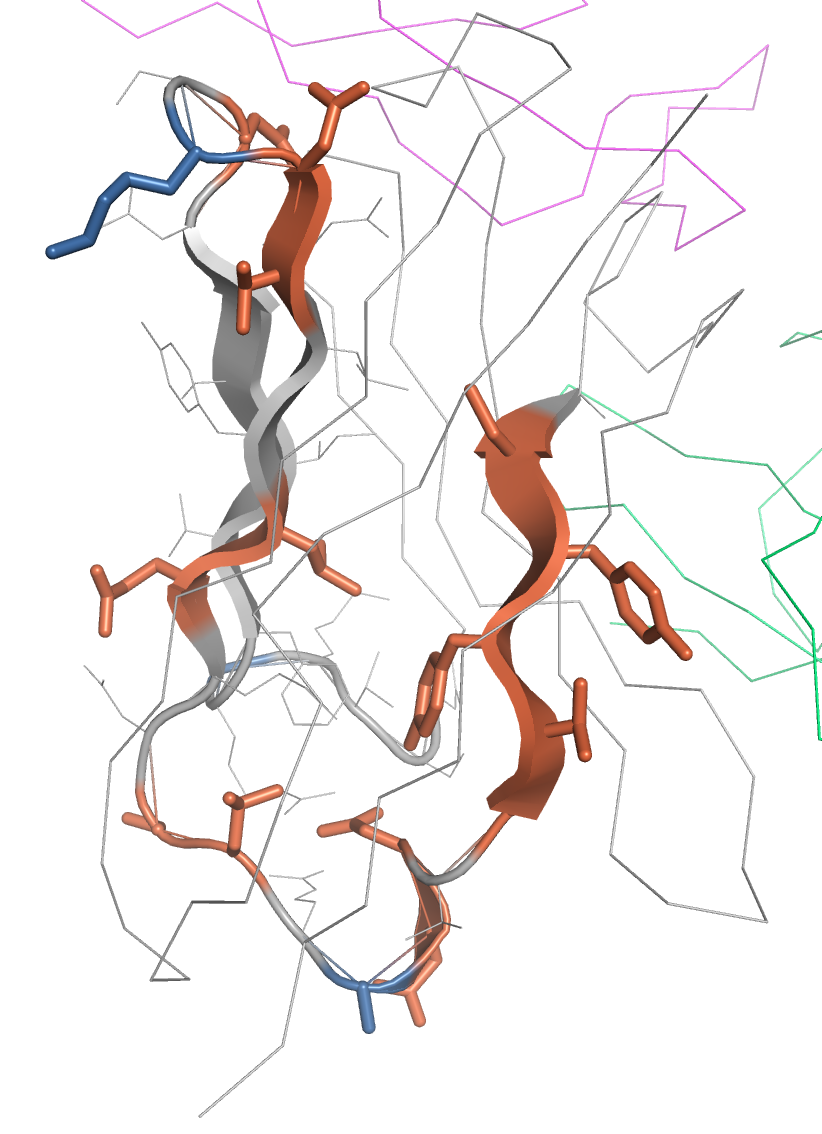
\includegraphics[width=1.5in]{bcell-structure.png}
  \caption{\
    Ribbon diagram of a sequenced portion of the heavy chain colored by selection inference.
    Purifying selection marked orange and diversifying selection marked blue.
    }
  \label{FIGbcell}
\end{marginfigure}

We have recently become very interested in the \textit{adaptive} immune system continually evolves within each individual in order to neutralize and destroy pathogens.
Specifically, we have embarked on a program to bring modern model-based statistical inference to the within-host evolution of antibody-making B cells.
Although the elements of B cell affinity maturation are the same as molecular evolution in other settings in being based on recombination, point mutation, and selection, there are some important differences with other settings.
Postdoc Duncan Ralph and I are approaching VDJ rearrangement group inference using pair hidden Markov models, resulting in a Bayes factor that can be used for clustering.
I am approaching the very strong mutation context dependence of mutation by doing model inference using composite likelihood strategies developed for interacting particle systems (joint with Peter Ralph, USC).
We are pursuing new methods to do evolutionary selection inference in the setting of many reads of varying length\scite{McCoy}{2014}{http://arxiv.org/abs/1403.3066} and have applied them to the inference of selection happening on B cell receptor V gene (Figure~\ref{FIGbcell}).


\section{Using geometry to better integrate over phylogenetic trees}
\begin{marginfigure}%
  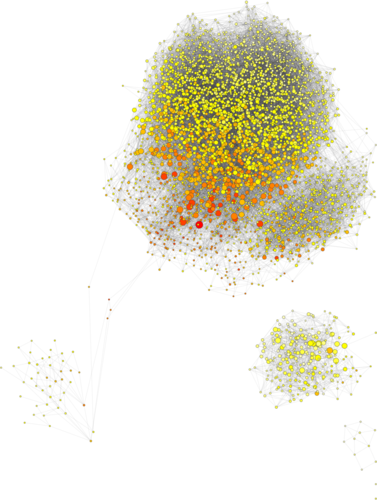
\includegraphics[width=1.5in]{ds6_small.png}
  \caption{\
    The collection of trees explored by an inference procedure.
    Vertices represent trees and edges represent SPR moves.
    Disconnected sets show peaks in the likelihood surface.
    }
  \label{FIGsprmix}
\end{marginfigure}
All model-based phylogenetic inference methods start with a heuristically constructed tree and then proceed by a series of random modifications of the tree whereby jumps to better (higher likelihood) trees are favored over jumps to lower likelihood trees.
Although there are certain guarantees concerning how phylogenetic reconstruction methods will perform if run for an infinite period of time, rather little is known about how these methods work when run for a finite period of time.
For example, there may be two ``peaks'' of good phylogenetic trees separated by a ``trough''; it may take an arbitrarily long time to cross between the peaks with high probability (Figure~\ref{FIGsprmix}).
Such behavior will manifest itself in overconfidence in the tree represented by the first peak selected.

Thus, in order to make confident statements it is necessary to gain an understanding of how these likelihood surfaces look on real data.
Postdoc Chris Whidden and I have explored these surfaces by equipping the collection of trees with a geometry corresponding to \textit{subtree-prune-regraft (SPR)} moves.
In this move, part of a tree is detached and then re-attached at another location.
These SPR moves are the canonical example of the type of tree modification done in phylogenetic inference as described above.

Our work enables analysis of the proximate causes of bad behavior of phylogenetic inference procedures by finding peaks and troughs in a graph representation of the set of phylogenetic trees\scite{Whidden}{2014}{http://arxiv.org/abs/1405.2120}.
We are now learning the ultimate causes of difficulty of movement in the SPR graph by quantifying large-scale features of the graph, and in the process characterized the symmetries of this graph induced by relabeling pairs of trees.
We are also exploring the degree to which conflicting signals in sequence alignments may contribute to such problems.


\section{Incorporating phylogenetic structure into ecological analysis}



\section{Software}

pakage to run software with nested parameter choices \scite{McCoy}{2013}{http://dx.doi.org/10.1093/bioinformatics/bts696}


% \bibliography{research}
% \bibliographystyle{unsrt}

\end{document}

\begin{marginfigure}%
  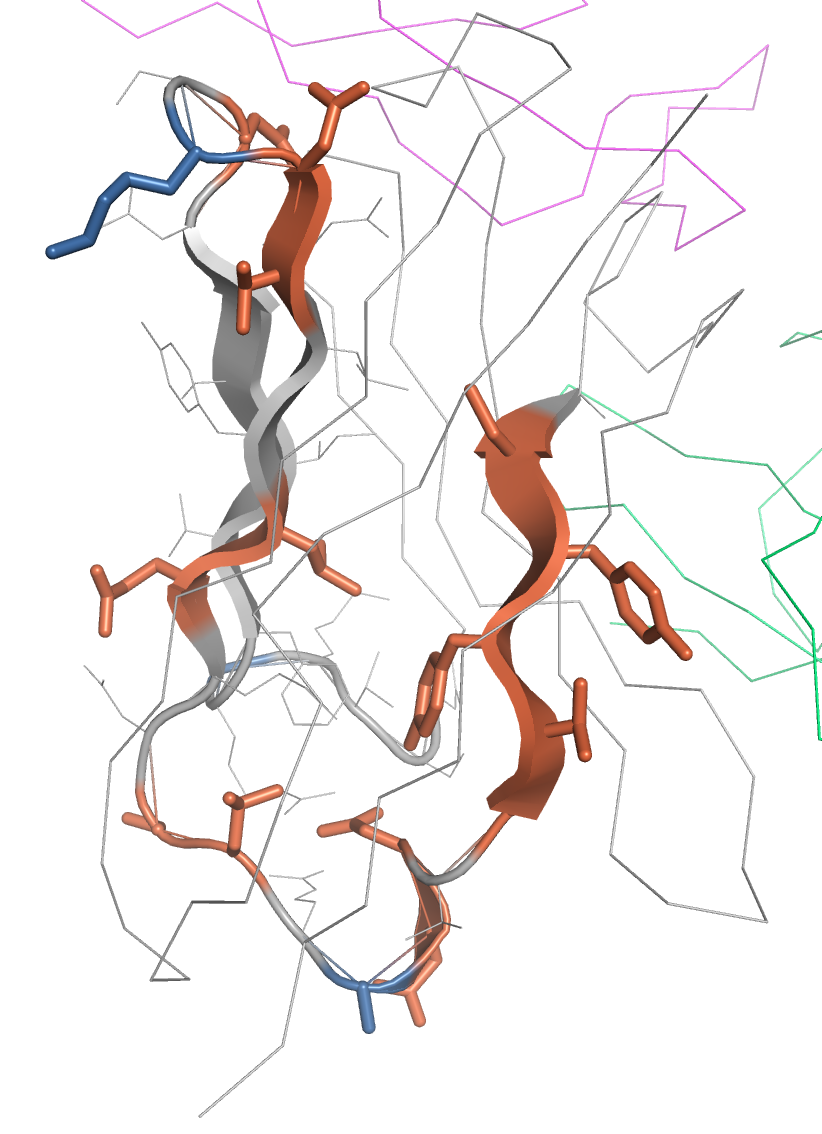
\includegraphics[width=2in]{bcell-structure.png}
  \caption{\
    Overview of B cell development.
    B cells first go through a combinatorial \emph{rearrangement} process resulting in a na\"ive B cell with single V, D, and J genes joined together by \emph{non-templated insertions}.
    These na\"ive cells then go through a Darwinian \emph{affinity maturation} process of mutation and selection to improve the affinity of the B cell receptor displayed on the outside of the cell.
    }
  \label{FIGoverview}
\end{marginfigure}

\begin{figure}[h]
  % \includegraphics[width=\linewidth]{selection.pdf}
  \caption{\
    An example per-site selection profile for a single individual; full figure and complete explanation available in our preprint.
    Upper panel: "violin" density plot of selection pressure $\omega$ for sites at various positions of the immunoglobulin heavy chain locus; $\omega > 1$ indicates diversifying selection, whereas $\omega < 1$ indicates purifying selection.
    Lower panel: counts of sites at various sites and their classification in terms of selection class.
    }
  \label{FIGselection}
\end{figure}


